\documentclass[a4]{article}
\pagestyle{myheadings}

%%%%%%%%%%%%%%%%%%%
% Packages/Macros %
%%%%%%%%%%%%%%%%%%%
\usepackage{mathrsfs}


\usepackage{fancyhdr}
\pagestyle{fancy}
\lhead{}
\chead{}
\rhead{}
\lfoot{}
\cfoot{} 
\rfoot{\normalsize\thepage}
\renewcommand{\headrulewidth}{0pt}
\renewcommand{\footrulewidth}{0pt}
\newcommand{\RomanNumeralCaps}[1]
{\MakeUppercase{\romannumeral #1}}

\usepackage{amssymb,latexsym}  % Standard packages
\usepackage[utf8]{inputenc}
\usepackage[russian]{babel}
\usepackage{MnSymbol}
\usepackage{amsmath,amsthm}
\usepackage{indentfirst}
\usepackage{graphicx}%,vmargin}
\usepackage{graphicx}
\graphicspath{{pictures/}} 
\usepackage{verbatim}
\usepackage{color}









\DeclareGraphicsExtensions{.pdf,.png,.jpg}% -- настройка картинок

\usepackage{epigraph} %%% to make inspirational quotes.
\usepackage[all]{xy} %for XyPic'a
\usepackage{color} 
\usepackage{amscd} %для коммутативных диграмм


\newtheorem{Lemma}{Лемма}[section]
\newtheorem{Proposition}{Предложение}[section]
\newtheorem{Theorem}{Теорема}[section]
\newtheorem{Corollary}{Следствие}[section]
\newtheorem{Remark}{Замечание}[section]
\newtheorem{Definition}{Определение}[section]
\newtheorem{Designations}{Обозначение}[section]




%%%%%%%%%%%%%%%%%%%%%%%% 
%Сношение с оглавлением% 
%%%%%%%%%%%%%%%%%%%%%%%% 
\usepackage{tocloft} 
\renewcommand{\cftdotsep}{2} %частота точек
\renewcommand\cftsecleader{\cftdotfill{\cftdotsep}}
\renewcommand{\cfttoctitlefont}{\hspace{0.38\textwidth} \LARGE\bfseries} 
\renewcommand{\cftsecaftersnum}{.}
\renewcommand{\cftsubsecaftersnum}{.}
\renewcommand{\cftbeforetoctitleskip}{-1em} 
\renewcommand{\cftaftertoctitle}{\mbox{}\hfill \\ \mbox{}\hfill{\footnotesize Стр.}\vspace{-0.5em}} 
\renewcommand{\cftsubsecfont}{\hspace{1pt}} 
\renewcommand{\cftparskip}{3mm} %определяет величину отступа в оглавлении
\setcounter{tocdepth}{5} 




\addtolength{\textwidth}{0.7in}
\textheight=630pt
\addtolength{\evensidemargin}{-0.4in}
\addtolength{\oddsidemargin}{-0.4in}
\addtolength{\topmargin}{-0.4in}

\newcommand{\empline}{\mbox{}\newline} 
\newcommand{\likechapterheading}[1]{ 
	\begin{center} 
		\textbf{\MakeUppercase{#1}} 
	\end{center} 
	\empline} 

\makeatletter 
\renewcommand{\@dotsep}{2} 
\newcommand{\l@likechapter}[2]{{\bfseries\@dottedtocline{0}{0pt}{0pt}{#1}{#2}}} 
\makeatother 
\newcommand{\likechapter}[1]{ 
	\likechapterheading{#1} 
	\addcontentsline{toc}{likechapter}{\MakeUppercase{#1}}} 





\usepackage{xcolor}
\usepackage{hyperref}
\definecolor{linkcolor}{HTML}{000000} % цвет ссылок
\definecolor{urlcolor}{HTML}{AA1622} % цвет гиперссылок

\hypersetup{pdfstartview=FitH,  linkcolor=linkcolor,urlcolor=urlcolor, colorlinks=true}



\def \newstr {\medskip \par \noindent} 



\begin{document}
	\def\contentsname{\LARGE{Содержание}}
	\thispagestyle{empty}
	\begin{center} 
		\vspace{2cm} 
		{\Large \sc Санкт-Петербургский Политехнический Университет}\\
		\vspace{2mm}
		{\Large\sc Петра Великого}\\
		\vspace{1cm}
		{\large \sc Институт прикладной математики и механики\\ 
			\vspace{0.5mm}
			\textsc{}}\\ 
		\vspace{0.5mm}
		{\large\sc Кафедра $"$Прикладная математика$"$}\\
		\vspace{15mm}
		
		
		{\sc \textbf{Отчёт\\
			Лабораторная работа №$3$\\
			по дисциплине\\
			"Математическая статистика"}
			\vspace{6mm}
			
		}
		\vspace*{2mm}
		
		
		\begin{flushleft}
			\vspace{4cm}
			\sc Выполнил студент:\\
			\sc Салихов С.Р.\\
			\sc группа: 3630102/70401\\
			\vspace{1cm}
			\sc Проверил:\\
			\sc к.ф-м.н., доцент\\
			\sc Баженов Александр Николавич
			\vspace{20mm}
		\end{flushleft}
	\end{center} 
	\begin{center}
		\vfill {\large\textsc{Санкт-Петербург}}\\ 
		2020 г.
	\end{center}
	
	\newpage
	\pagestyle{plain}
	
	%\begin{center}
	%\begin{abstract} 
	
	%\end{abstract}
	
	%\end{center}
	
	\newpage
	\tableofcontents{}
	\newpage
	\listoffigures
	\newpage
	\listoftables
	\newpage
	
	
	\section{Постановка задачи}
	
	Для 5-ти рапределений:\\
		Нормальное распределение $N(x,0,1)$\\
		Распределение Коши $C(x,0,1)$\\
		Распределение Лапласа $L( x,0,\frac{1}{\sqrt{2}})$\\
		Распределение Пуассона $P(k, 10)$\\
		Равномерное Распределение $U(x,-\sqrt{3}, \sqrt{3})$\\
		
		Сгенерировать выборки размером 20, и 100 элементов.\\
		Построить для них боксплот Тьюки.\\
		Для каждого распределения определить долю выбросов эксперементально(сгенерировав выборку, соответствующую распределению 1000 раз и вычислив среднюю долю выбросов) и сравнить с результатами полученными теоретически.
		
	
	\section{Теория}
		\subsection{Распределения}
		
			\begin{equation}\label{eqn:normal}
			N(x,0,1) = \frac{1}{\sqrt{2\pi}}e^{-\frac{x^2}{2}}
			\end{equation} 
			
			\begin{equation}\label{eqn:cauchy}
			C(x,0,1) = \frac{1}{\pi(1+x^2)}
			\end{equation}
			
			\begin{equation}\label{eqn:laplace}
			L\left( x,0,\frac{1}{\sqrt{2}}\right) = \frac{1}{\sqrt{2}}e^{-\sqrt{2}\vert x\vert}
			\end{equation}
			
			\begin{equation}\label{eqn:poisson}
			P(k,10) = \frac{10^k}{k!}e^{-10}
			\end{equation}  
			
			\begin{equation}\label{eqn:uniform}
			U(x,-\sqrt{3}, \sqrt{3}) = 
			\begin{cases}
			\frac{1}{2\sqrt{3}} &\vert x\vert \leqslant \sqrt{3}\\
			0 &\vert x\vert > \sqrt{3}
			\end{cases}
			\end{equation}
		
		\subsection{Гистограмма}
			\subsubsection{Определение}
				Боксплот (англ. box plot) — график, использующийся в описательной статистике, компактно изображающий одномерное распределение вероятностей.
		
			\subsubsection{Описание}
				Такой вид диаграммы в удобной форме показывает медиану, нижний и верхний квартили и выбросы. Несколько таких ящиков можно нарисовать бок
				о бок, чтобы визуально сравнивать одно распределение с другим; их можно располагать как горизонтально, так и вертикально. Расстояния между
				различными частями ящика позволяют определить степень разброса (дисперсии) и асимметрии данных и выявить выбросы.
			\subsubsection{Использование}
				Границами ящика служат первый и третий квартили, линия в середине
				ящика — медиана. Концы усов — края статистически значимой выборки
				(без выбросов). Длину «усов» определяют разность первого квартиля и полутора межквартильных расстояний и сумма третьего квартиля и полутора
				межквартильных расстояний. Формула имеет вид:\\
				$$X_1 = Q_1 - \frac{3}{2}(Q_3 - Q_1), X_2 = Q_3 + \frac{3}{2}(Q_3 - Q_1)$$
				Где $X_1$ - нижняя граница уса, $X_2$ - верхняя граица уса, $Q_1$ - первый квартиль, $Q_3$ - третий квартиль.\\
				Данные, выходящие за границы усов (выбросы), отображаются на графике
				в виде маленьких кружков.
	\section{Реализация}
	Для генерации выборки был использован $Python\;3.7$: модуль $random$ библиотеки $numpy$ для генерации случайных чисел с различными распределениями. Боксплот Тьюки был построен средствами $matplotlib$.
	\newpage
	\section{Результаты}
		\subsection{Боксплот Тьюки}
		Ввелём на оси y следующие обозначения:\\
		1 соответствует выборке из 20-ти элементов\\
		2 - соответствует выборке из 100 элементов\\
			\begin{center}
				
				\begin{figure}[h]
					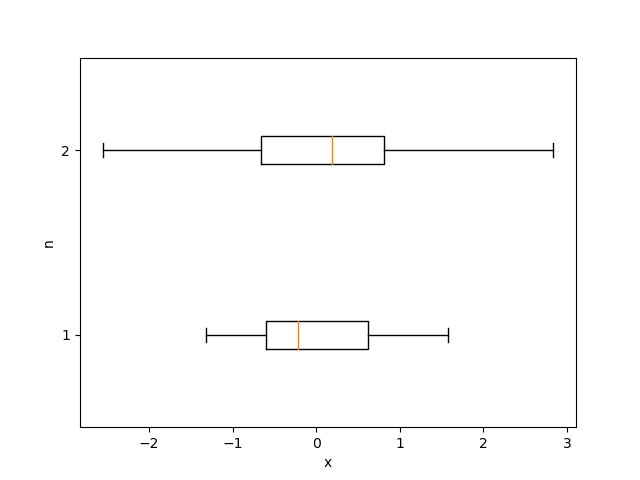
\includegraphics[width=\textwidth]{normal.png} 
					\caption[Нормальное распределение]{Нормальное распределение}
				\end{figure}
				\newpage
				\begin{figure}[h]
					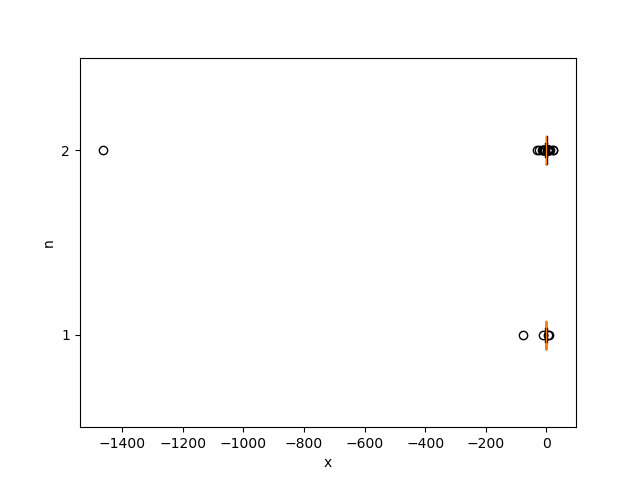
\includegraphics[width=\textwidth]{cauchy.png}
					\caption[Распределение Коши]{Распределение Коши}
				\end{figure}
				\newpage
				\begin{figure}[h]
					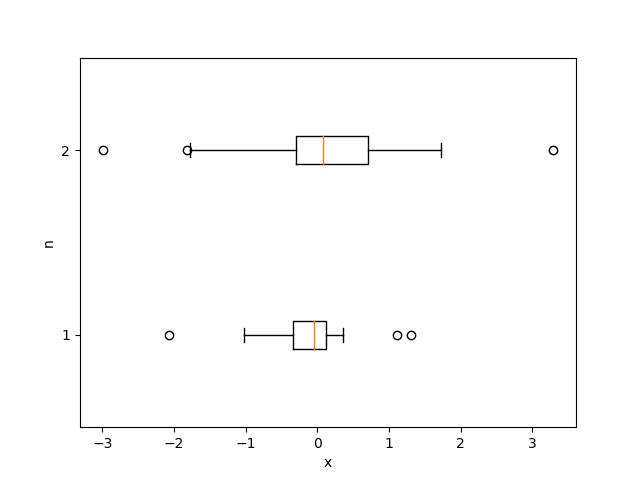
\includegraphics[width=\textwidth]{laplace.png}
					\caption[Распределение Лапласа]{Распределение Лапласа}
				\end{figure}
				\newpage
				\begin{figure}[h]
					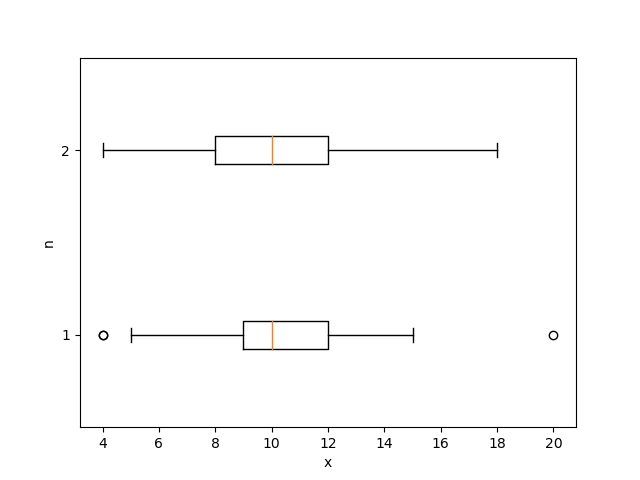
\includegraphics[width=\textwidth]{poisson.png}
					\caption[Распределение Пуассона]{Распределение Пуассона}
				\end{figure}
				\newpage
				\begin{figure}[h]
					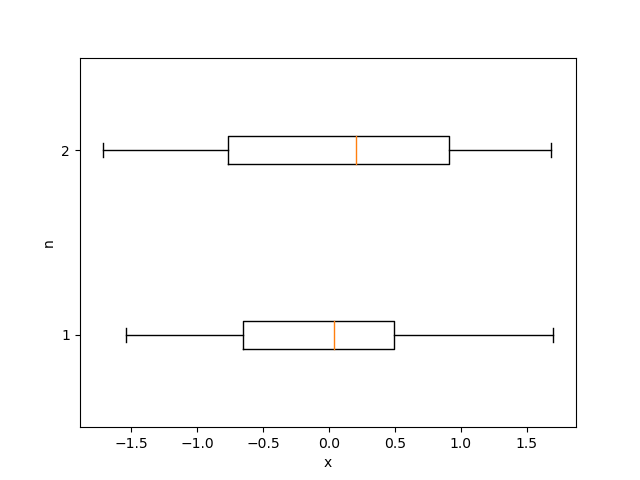
\includegraphics[width=\textwidth]{uniform.png}
					\caption[Равномерное распределение]{Равномерное распределение}
				\end{figure}
	
		\end{center}
		\newpage
		\begin{table}[h]
			
			\caption{Выбросы различных распределений в зависимости от выборки}
			\label{tab:my_label}
			\begin{center}
				\vspace{5mm}
				\begin{tabular}{|c|c|}
					\hline
					Выборка & Процент выбросов\\
					\hline
					Нормальное	&\\
					\hline
					n = 20   & 	2    \\
					\hline
					n = 100   &	1    \\
					\hline
					Коши	&\\
					\hline
					n = 20   & 	15    \\
					\hline
					n = 100  & 	15    \\
					\hline
					Лапласа	&\\
					\hline
					n = 20    &	7    \\
					\hline
					n = 100   &	6    \\
					\hline
					Пуассона	&\\
					\hline
					n = 20   & 	3    \\
					\hline
					n = 100  & 	1    \\
					\hline
					Равномерное	&\\
					\hline
					n = 20    &	0    \\
					\hline
					n = 100   &	0   \\ 
					\hline
				\end{tabular}
				
			\end{center}
			
		\end{table}
		
	\newpage
	\section{Обсуждение}
		\subsection{Анализ данных}
		Из экспериментально полученных данных можно вывести соотношение между процентами выбросов:\\
		равномерное распределение < нормальное распределение < распределение Пуассона < распределение Лапласа < распределение Коши
		\subsection{Сравнение с теоретическими значениями}
		Полученные экспериментально данные близки к теоретическим и видно, что наименьший процент выбросов у равномерного распределения ,а наибольший у распределения Коши
	
	\section{Литература}
	
	\href{https://physics.susu.ru/vorontsov/language/numpy.html}{Модуль numpy}
	
	\href{https://matplotlib.org/3.1.1/api/_as_gen/matplotlib.pyplot.boxplot.html}{matplotlib boxplot}
	
	\href{https://habr.com/ru/post/267123/}{Боксплот Тьюки}
	
	\section{Приложения}
	
	\href{https://github.com/LuciusGen/Matstat/blob/master/Lab3/lab3.py}{Код лаборатрной}
	
	\href{https://github.com/LuciusGen/Matstat/blob/master/Lab3/lab3.tex}{Код отчёта}
	
\end{document}